\chapter{Parade}
\spp{
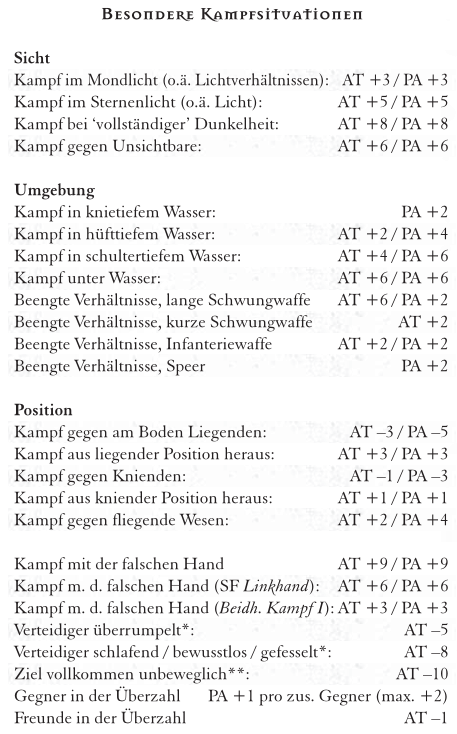
\includegraphics[width=0.9\linewidth]{Kampf/Home/kampfsituationen.png}\\
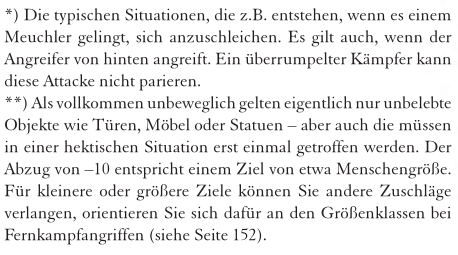
\includegraphics[width=0.9\linewidth]{Kampf/Home/kampfsituationenkommentar.png}
}{
\begin{center}
    \begin{tikzpicture}[node distance = 3cm, auto]
            % Nodes
        \node [block] (init) {\hylt{parade}{paradestart}{Wird angegriffen}} ;
        \node [decision, below of=init] (dec) {Kann parieren?};
        \node [block, right = 1cm of dec] (hit) {\hylin{treffer}{Treffer}};
        \node [decision, below of=dec] (pardec) {Parieren?};
        \node [block, below left of=pardec] (par) {Manöver wählen*:\\\hylin{abwehrkarten}{Parade}};
        \node [block, below right of=pardec] (ausw) {\hylin{ausweichen}{Ausw.}};
        \node [block, below = 3cm of pardec] (end) {\hylin{schaden}{Treffer}};

            % Edges
        \path [line] (init) -> (dec);
        \path [line] (dec) ->node [left] {Ja} (pardec);
        \path [line] (dec) ->node [above] {Nein} (hit);
        \path [line] (pardec) ->node {Nein} (ausw);
        \path [line] (pardec) ->node[above left] {Ja}(par);
        \path [line] (par) -> node[below left] {Nein} (end);
        \path [line] (ausw) -> node[below right] {Nein} (end);
    \end{tikzpicture}\\
\end{center}
*) Einen \textbf{Gezielten Schlag} zu parieren ist um -2 (Bauch/Brust), -4
*(Kopf) erleichtert. Mit \textit{Aufmerksamkeit} um zusätzlich -2.

Eine \textbf{Parade} muss vor auswürfeln der \textbf{Attacke} angesagt
werden. Bei misslingen der Attacke \textbf{verfällt } die Parade. Sonst wäre
reaktives Kämpfen zu stark.
}